% The methods that you use goes here
{\large\underline{\textbf{Problém batohu 0/1}}} \\[0.5em]
Každá položka může být vybrána nejvýše jednou tak, aby celková hodnota vybrané podmnožiny položek byla maximální a součet jejich vah nepřesáhl kapacitu batohu.
\begin{equation}
  \max \sum_{i=1}^{n} v_i x_i
  \quad \text{s podmínkou} \quad \sum_{i=1}^{n} w_i x_i \leq C,
  \quad x_i \in \{0,1\}
\end{equation}

{\large\underline{\textbf{Kvantová reprezentace řešení}}} \\[0.5em]
V binárním \emph{QIEA} je qubit (jedinec) popsán dvojicí koeficientů $\alpha$ a $\beta$, přičemž systém složený z $m$ qubitů (populace) lze vyjádřit jako:
\label{eq:quantum-representation} 
\begin{equation}
  \begin{bmatrix}
    \alpha_1 & \alpha_2 & \dots & \alpha_m \\ \beta_1 & \beta_2 & \dots & \beta_m
  \end{bmatrix},
  \quad \text{kde} \quad \forall i \in \left\{ 1,2,\dots,m \right\}: \quad \alpha_i^2 + \beta_i^2 = 1.
\end{equation}
Pravděpodobnostní koeficienty $\alpha_i$ a $\beta_i$ $i$-tého qubitu jsou aktualizovány pomocí kvantového rotačního hradla, viz obrázek~\ref{fig:rotation-gate}:
\begin{equation}
  \label{eq:rotation-gate-angles}
  \begin{bmatrix} 
    \alpha_i' \\ 
    \beta_i'
  \end{bmatrix} = 
  \begin{bmatrix} 
    \cos{\left( \Delta\theta_i \right)} & - \sin{\left( \Delta\theta_i \right)} \\
    \sin{\left( \Delta\theta_i \right)} & \cos{\left( \Delta\theta_i \right)}
  \end{bmatrix} 
  \begin{bmatrix} 
    \alpha_i \\ 
    \beta_i 
  \end{bmatrix},
\end{equation}
kde je úhel $\Delta\theta_i$ určen ná základě tabulky~\ref{tab:look-up-table-Delta}, a to podle aktuálně pozorovaného řešení $x_i$ a nejlepšího známého řešení $b_i$:

\begin{minipage}{0.49\linewidth}
    \centering
    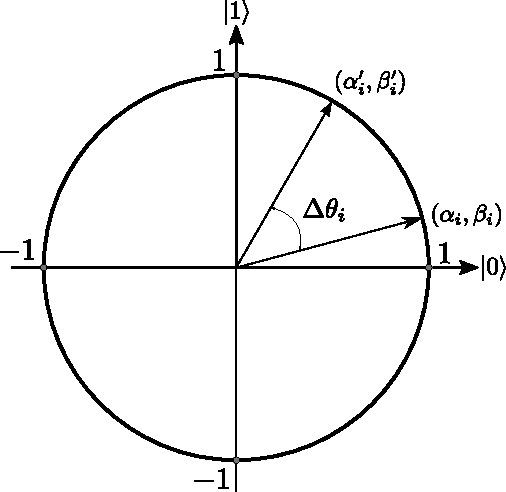
\includegraphics[width=0.9\linewidth]{rotation-gate.pdf}
    \captionof{figure}{Rotační hradlo.}
    \label{fig:rotation-gate}
\end{minipage}
\hfill
\begin{minipage}{0.49\linewidth}
    \centering
    \begin{tabular}{c c|c}
    \toprule
    $x_i$ & $b_i$ & $\Delta\theta_i$ \\
    \midrule
    1 & 1 & 0 \\
    0 & 1 & $a$ \\
    0 & 0 & 0 \\
    1 & 0 & $-a$ \\
    \bottomrule
    \end{tabular}
    \captionof{table}{Tabulka pro odvození $\Delta\theta_i$.}
    \label{tab:look-up-table-Delta}
\end{minipage}

\vspace{0.5em}

{\large\underline{\textbf{Použité algoritmy}}} \\[0.5em]
V rámci experimentální části byly testovány čtyři \emph{QIEA}:
\begin{itemize}
  \item \emph{QIGA} (kvantově inspirovaný genetický algoritmus),
  \item \emph{QISA} (kvantově inspirované simulované žíhání),
  \item \emph{QSE} (kvantově inspirovaný částicový roj)
  \item a vlastní navržená varianta \emph{QIPSO} vycházející z \emph{QSE}.
\end{itemize}
Cílem bylo porovnat jejich schopnost řešit problém batohu 0/1 při různých velikostech instancí.
Pro shrnutí parametrů testovaní vizte tabulka~\ref{tab:experiment-settings}.

\vspace{0.5em}

\begin{minipage}{\linewidth}
  \centering
  \begin{tabular}{|l|l|}
  \hline
  \textbf{Položka} & \textbf{Hodnota} \\
  \hline
  Testované algoritmy & QIGA, QISA, QSE, QIPSO \\
  \hline
  Instance & 100, 250, 500, 1000, 2000, 5000 položek \\
  \hline
  Počet běhů & 30 na každé nastavení \\
  \hline
  Fitness evaluací & 10 000 na běh \\
  \hline
  \end{tabular}
  \captionof{table}{Parametry experimentálního nastavení.}
  \label{tab:experiment-settings}
\end{minipage}
\vspace{0.5em}
